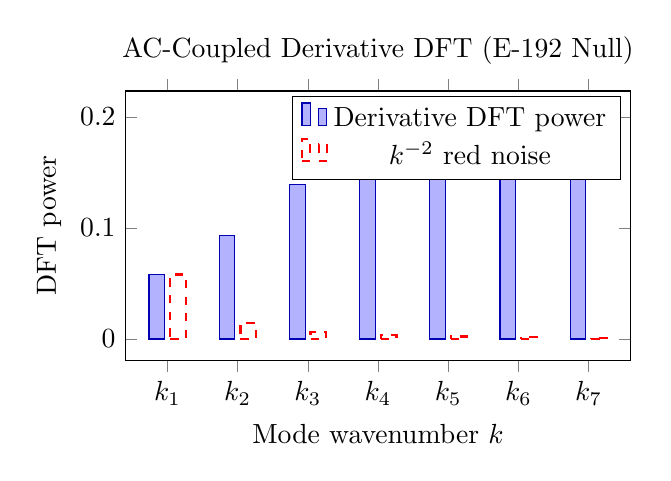
\begin{tikzpicture}
\begin{axis}[
  xlabel={Mode wavenumber $k$},
  ylabel={DFT power},
  width=8cm, height=5cm,
  ybar, bar width=0.2,
  xtick={0.898,1.795,2.693,3.590,4.488,5.386,6.283},
  xticklabels={$k_1$,$k_2$,$k_3$,$k_4$,$k_5$,$k_6$,$k_7$},
  title={AC-Coupled Derivative DFT (E-192 Null)}
]
\addplot[blue!70!black,fill=blue!30] coordinates {(0.8976,0.058046) (1.7952,0.093490) (2.6928,0.139474) (3.5904,0.180744) (4.4880,0.203266) (5.3856,0.198692) (6.2832,0.167058)};
\addplot[red,dashed,thick,mark=none] coordinates {(0.8976,0.058046) (1.7952,0.014512) (2.6928,0.006450) (3.5904,0.003628) (4.4880,0.002322) (5.3856,0.001612) (6.2832,0.001185)};
\legend{Derivative DFT power,$k^{-2}$ red noise}
\end{axis}
\end{tikzpicture}
